\documentclass{standalone}
\usepackage{tikz}
\usetikzlibrary{patterns, positioning}


\begin{document}
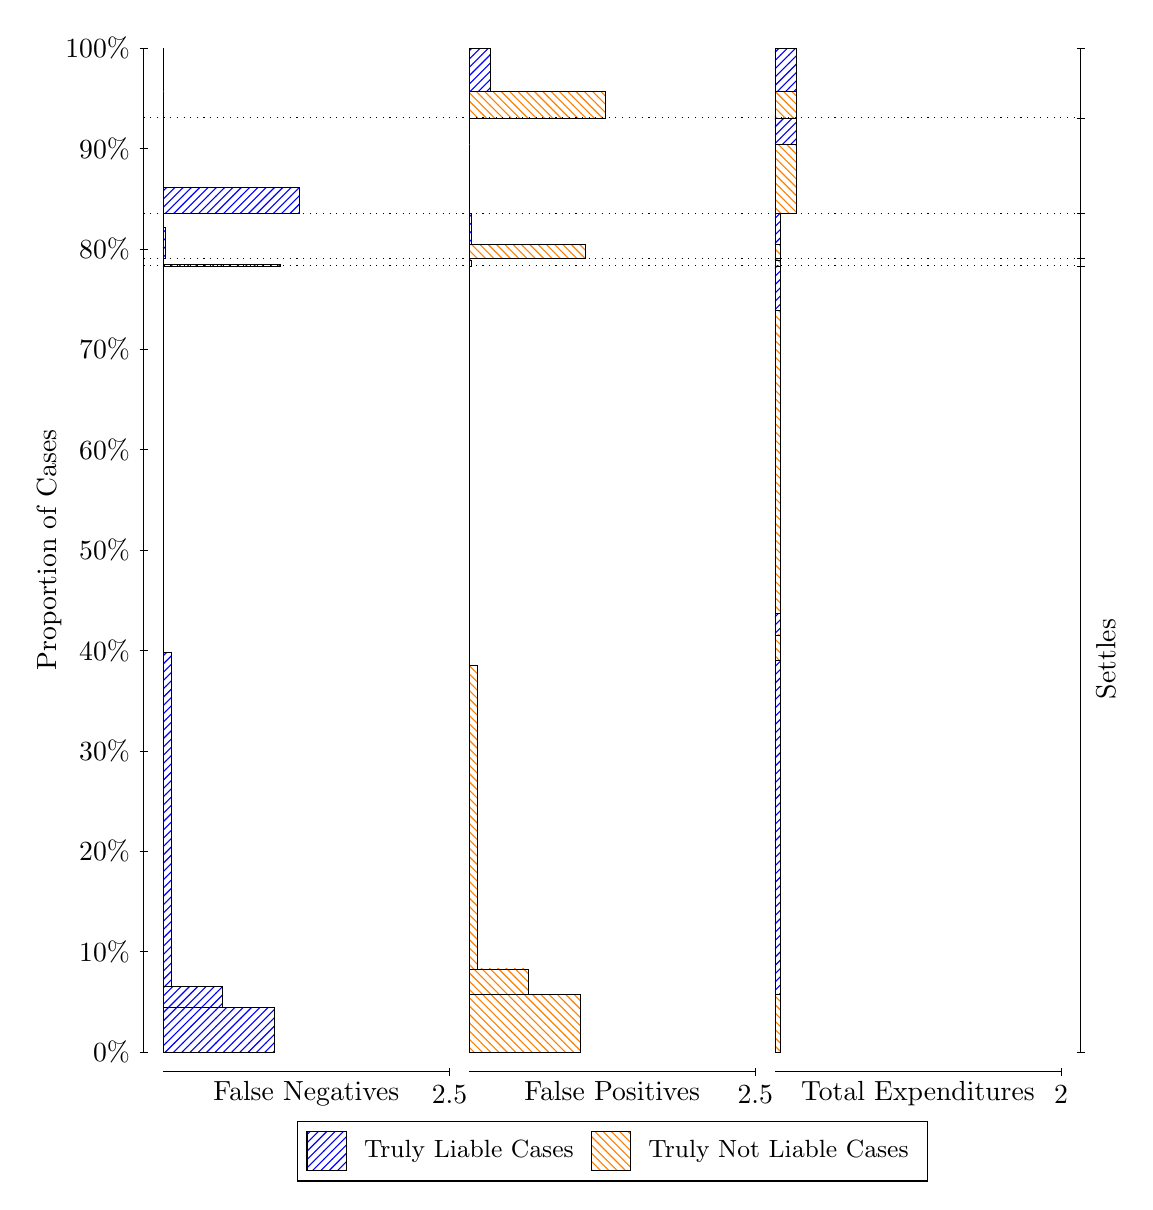
\begin{tikzpicture}
\draw[black, very thin] (1.5,1.75) -- (1.5,14.5);
\node[rotate=90, text=black, anchor=center] at (0.3, 8.125) {Proportion of Cases};
\draw[black, very thin] (1.45,1.75) -- (1.55,1.75);
\node[text=black, anchor=east] at (1.45, 1.75) {0\%};
\draw[black, very thin] (1.45,3.025) -- (1.55,3.025);
\node[text=black, anchor=east] at (1.45, 3.025) {10\%};
\draw[black, very thin] (1.45,4.3) -- (1.55,4.3);
\node[text=black, anchor=east] at (1.45, 4.3) {20\%};
\draw[black, very thin] (1.45,5.575) -- (1.55,5.575);
\node[text=black, anchor=east] at (1.45, 5.575) {30\%};
\draw[black, very thin] (1.45,6.85) -- (1.55,6.85);
\node[text=black, anchor=east] at (1.45, 6.85) {40\%};
\draw[black, very thin] (1.45,8.125) -- (1.55,8.125);
\node[text=black, anchor=east] at (1.45, 8.125) {50\%};
\draw[black, very thin] (1.45,9.4) -- (1.55,9.4);
\node[text=black, anchor=east] at (1.45, 9.4) {60\%};
\draw[black, very thin] (1.45,10.675) -- (1.55,10.675);
\node[text=black, anchor=east] at (1.45, 10.675) {70\%};
\draw[black, very thin] (1.45,11.95) -- (1.55,11.95);
\node[text=black, anchor=east] at (1.45, 11.95) {80\%};
\draw[black, very thin] (1.45,13.225) -- (1.55,13.225);
\node[text=black, anchor=east] at (1.45, 13.225) {90\%};
\draw[black, very thin] (1.45,14.5) -- (1.55,14.5);
\node[text=black, anchor=east] at (1.45, 14.5) {100\%};

\draw[black, very thin] (13.4,1.75) -- (13.4,14.5);
\draw[black, very thin] (13.35,1.75) -- (13.45,1.75);
\node[anchor=west] at (13.35, 1.75) {};
\draw[black, very thin] (13.35,11.733) -- (13.45,11.733);
\node[anchor=west] at (13.35, 11.733) {};
\draw[black, very thin] (13.35,11.832) -- (13.45,11.832);
\node[anchor=west] at (13.35, 11.832) {};
\draw[black, very thin] (13.35,12.398) -- (13.45,12.398);
\node[anchor=west] at (13.35, 12.398) {};
\draw[black, very thin] (13.35,13.613) -- (13.45,13.613);
\node[anchor=west] at (13.35, 13.613) {};
\draw[black, very thin] (13.35,14.5) -- (13.45,14.5);
\node[anchor=west] at (13.35, 14.5) {};

\draw[black, very thin, pattern color=blue, pattern=north east lines] (1.75,1.75) rectangle (3.1579,2.312);
\draw[black, very thin, pattern color=blue, pattern=north east lines] (1.75,2.312) rectangle (2.5039,2.5836);
\draw[black, very thin, pattern color=blue, pattern=north east lines] (1.75,2.5836) rectangle (1.8499,6.8244);
\draw[black, very thin, pattern color=orange, pattern=north west lines] (1.75,6.8244) rectangle (1.75,11.733);
\draw[black, very thin, pattern color=blue, pattern=north east lines] (1.75,11.733) rectangle (3.2306,11.756);
\draw[black, very thin, pattern color=orange, pattern=north west lines] (1.75,11.756) rectangle (1.75,11.832);
\draw[black, very thin, pattern color=blue, pattern=north east lines] (1.75,11.832) rectangle (1.7773,12.223);
\draw[black, very thin, pattern color=orange, pattern=north west lines] (1.75,12.223) rectangle (1.75,12.398);
\draw[black, very thin, pattern color=blue, pattern=north east lines] (1.75,12.398) rectangle (3.4758,12.734);
\draw[black, very thin, pattern color=orange, pattern=north west lines] (1.75,12.734) rectangle (1.75,13.613);
\draw[black, very thin, pattern color=orange, pattern=north west lines] (1.75,13.613) rectangle (1.75,13.949);
\draw[black, very thin, pattern color=blue, pattern=north east lines] (1.75,13.949) rectangle (1.75,14.5);
\draw[black, very thin, pattern color=orange, pattern=north west lines] (5.6333,1.75) rectangle (7.0413,2.4797);
\draw[black, very thin, pattern color=orange, pattern=north west lines] (5.6333,2.4797) rectangle (6.3873,2.8065);
\draw[black, very thin, pattern color=orange, pattern=north west lines] (5.6333,2.8065) rectangle (5.7333,6.6584);
\draw[black, very thin, pattern color=blue, pattern=north east lines] (5.6333,6.6584) rectangle (5.6333,11.733);
\draw[black, very thin, pattern color=orange, pattern=north west lines] (5.6333,11.733) rectangle (5.6606,11.809);
\draw[black, very thin, pattern color=blue, pattern=north east lines] (5.6333,11.809) rectangle (5.6333,11.832);
\draw[black, very thin, pattern color=orange, pattern=north west lines] (5.6333,11.832) rectangle (7.1139,12.007);
\draw[black, very thin, pattern color=blue, pattern=north east lines] (5.6333,12.007) rectangle (5.6606,12.398);
\draw[black, very thin, pattern color=orange, pattern=north west lines] (5.6333,12.398) rectangle (5.6333,13.277);
\draw[black, very thin, pattern color=blue, pattern=north east lines] (5.6333,13.277) rectangle (5.6333,13.613);
\draw[black, very thin, pattern color=orange, pattern=north west lines] (5.6333,13.613) rectangle (7.3592,13.949);
\draw[black, very thin, pattern color=blue, pattern=north east lines] (5.6333,13.949) rectangle (5.9058,14.5);
\draw[black, very thin, pattern color=orange, pattern=north west lines] (9.5167,1.75) rectangle (9.5848,2.4797);
\draw[black, very thin, pattern color=blue, pattern=north east lines] (9.5167,2.4797) rectangle (9.5848,6.7206);
\draw[black, very thin, pattern color=orange, pattern=north west lines] (9.5167,6.7206) rectangle (9.5848,7.0473);
\draw[black, very thin, pattern color=blue, pattern=north east lines] (9.5167,7.0473) rectangle (9.5848,7.3188);
\draw[black, very thin, pattern color=orange, pattern=north west lines] (9.5167,7.3188) rectangle (9.5848,11.171);
\draw[black, very thin, pattern color=blue, pattern=north east lines] (9.5167,11.171) rectangle (9.5848,11.733);
\draw[black, very thin, pattern color=orange, pattern=north west lines] (9.5167,11.733) rectangle (9.5848,11.809);
\draw[black, very thin, pattern color=blue, pattern=north east lines] (9.5167,11.809) rectangle (9.5848,11.832);
\draw[black, very thin, pattern color=orange, pattern=north west lines] (9.5167,11.832) rectangle (9.5848,12.007);
\draw[black, very thin, pattern color=blue, pattern=north east lines] (9.5167,12.007) rectangle (9.5848,12.398);
\draw[black, very thin, pattern color=orange, pattern=north west lines] (9.5167,12.398) rectangle (9.7892,13.277);
\draw[black, very thin, pattern color=blue, pattern=north east lines] (9.5167,13.277) rectangle (9.7892,13.613);
\draw[black, very thin, pattern color=orange, pattern=north west lines] (9.5167,13.613) rectangle (9.7892,13.949);
\draw[black, very thin, pattern color=blue, pattern=north east lines] (9.5167,13.949) rectangle (9.7892,14.5);
\draw[black, dotted] (1.5,11.733) -- (13.4,11.733);
\draw[black, dotted] (1.5,11.832) -- (13.4,11.832);
\draw[black, dotted] (1.5,12.398) -- (13.4,12.398);
\draw[black, dotted] (1.5,13.613) -- (13.4,13.613);
\draw[black, very thin] (1.75,1.5) -- (5.3833,1.5);
\node[text=black, anchor=north] at (3.5667, 1.5) {False Negatives};
\draw[black, very thin] (5.3833,1.45) -- (5.3833,1.55);
\node[text=black, anchor=north] at (5.3833, 1.45) {2.5};

\draw[black, very thin] (5.6333,1.5) -- (9.2667,1.5);
\node[text=black, anchor=north] at (7.45, 1.5) {False Positives};
\draw[black, very thin] (9.2667,1.45) -- (9.2667,1.55);
\node[text=black, anchor=north] at (9.2667, 1.45) {2.5};

\draw[black, very thin] (9.5167,1.5) -- (13.15,1.5);
\node[text=black, anchor=north] at (11.333, 1.5) {Total Expenditures};
\draw[black, very thin] (13.15,1.45) -- (13.15,1.55);
\node[text=black, anchor=north] at (13.15, 1.45) {2};

\node[text=black, centered, rotate=90] at (13.72, 6.7414) {Settles};





\draw (7.449999999999999,1.5) node[draw=none] (baseCoordinate) {};
\begin{scope}[align=center]
        \matrix[scale=0.5, draw=black, below=0.5cm of baseCoordinate, nodes={draw}, column sep=0.1cm]{
            \node[rectangle, draw, minimum width=0.5cm, minimum height=0.5cm, pattern color=blue, pattern=north east lines] {}; &
            \node[draw=none, font=\small, text=black] (B) {Truly Liable Cases}; &
            \node[rectangle, draw, minimum width=0.5cm, minimum height=0.5cm, pattern color=orange, pattern=north west lines] {}; &
            \node[draw=none, font=\small, text=black] (B) {Truly Not Liable Cases}; \\
            };
\end{scope}

\end{tikzpicture}
\end{document}